\documentclass[11pt]{article}

% Load custom style packages  
\usepackage{mystyle}
\usepackage{mycommands}

% Additional packages for tcolorboxes and enhanced content
\definecolor{cellbackground}{RGB}{248,248,248}
\definecolor{cellborder}{RGB}{200,200,200}

% Bibliography setup - point to the main references file
\addbibresource{../references.bib}

% Document metadata
\title{\class{}: Machine Learning Lecture Notes}
\author{\instructor{} \\ Columbia University}
\date{\semester{}}

\begin{document}

\maketitle

\tableofcontents
\newpage

% Chapter 1: Learning
\section{Learning}

\subsection{What is Machine Learning?}

I sometimes find the term ``machine learning'' to be frustrating. It sounds too impressive if you've already been running regressions to fulfill the modern duty to be data driven. Similarly, the use of words like ``model'' might frustrate you if you have a theorist's understanding of a model as a more complete description of behavior. But we come to machine learning on machine learning's terms, and this requires some language acquisition. Let's first get our arms around the idea of ``learning'' and ``machine learning,'' with the help of two foundational figures in the field.

Computer scientist Marvin Minsky offered the definition below, though with the preface that it was ``too broad to have much use.''

\begin{displayquote}
``Learning is making useful changes in our minds.''\\
--- \cite{minsky1986society}
\end{displayquote}

Computer scientist Tom Mitchell, in his widely cited textbook, provides a structured definition.

\begin{displayquote}
``Machine Learning is the study of computer algorithms that improve automatically through experience.''\\
--- \cite{mitchell1997machine}
\end{displayquote}

Mitchell's definition is common in the field and easily coexists with the idea of a well-posed learning problem, which we will introduce shortly. And there are less precise, but still useful definitions, like the one below from political scientists.

\begin{displayquote}
``Machine learning is a class of flexible algorithmic and statistical techniques for prediction and dimension reduction.''\\
--- \cite{grimmer2021machine}
\end{displayquote}

With these rough boundaries, we can discuss learning problems and their key similarities in taking data, ``learning'' from it to produce a line in the case of linear regression, or a fitted model more abstractly, all guided by some measure of what makes that the best fit. But how do we know when a problem is actually suitable for machine learning? Mitchell offers a more structured framework for identifying well-posed learning problems.

\subsection{Well-Posed Learning Problems}

\begin{definitionbox}[title={Machine Learning (Mitchell 1997)}]
A computer program is said to \textbf{learn} from experience \textit{E} with respect to some class of tasks \textit{T} and performance measure \textit{P}, if its performance at tasks in \textit{T}, as measured by \textit{P}, improves with experience \textit{E} \cite{mitchell1997machine}.
\end{definitionbox}

This definition provides a framework for thinking about learning problems, though it can be somewhat narrow. Not all useful ML techniques fit perfectly into this framework, as we will see.

\subsubsection{Example: Wage Prediction}

Consider a system that predicts wages based on education level:

\begin{itemize}
\item \textbf{Task T}: Predicting wages from years of education
\item \textbf{Performance measure P}: Mean squared error (MSE) between predicted and actual wages
\item \textbf{Training experience E}: Observing education-wage pairs from survey data
\end{itemize}

If we observe $i=1,\dots,n$ and make prediction $\hat{y}_i$ for all $i$, our performance measure is
\begin{equation}
\text{MSE} = \frac{1}{n}\sum_{i=1}^{n} (y_i -\hat{y}_i)^2
\label{eq:mse-basic}
\end{equation}
If we use a linear model, $\hat{y}_i=\hat{\beta}_0 + \hat{\beta}_1x_i$, then we are describing ordinary least squares.

\subsubsection{Example: Playing Board Games}

AlphaGo was trained to play Go by teaching itself. It used both supervised learning and self-play reinforcement learning.

\begin{itemize}
\item \textbf{Task T}: Playing the board game Go
\item \textbf{Performance measure P}: Percent of games won against opponents
\item \textbf{Training experience E}: Playing practice games against itself and against humans
\end{itemize}

Note that while AlphaGo's performance P is measured by win percentage, the actual training process optimizes a different objective that correlates with winning. P is an \textit{evaluation metric} and not necessarily what is optimized during training.

Famously, AlphaGo would go on to defeat the reigning grandmaster of Go in four of five matches. This was celebrated by the AI community and even Rick Rubin \cite{rubin2023creative}. The training experience, playing against itself, was advantageous because AlphaGo discovered a unique and unexpected way to play.

\subsection{Types of Learning Tasks}

We won't encounter many learning problems similar to playing Go in the social sciences. Instead, we'll see a lot of applications more similar to the wage prediction problem. Wage prediction is a case of \textit{supervised learning}.

Textbooks like \cite{james2023introduction} often introduce a \textit{supervised} vs \textit{unsupervised} dichotomy. We will follow that convention, but note that more complete taxonomies might include reinforcement learning or semi-supervised learning.

\subsubsection{Supervised Learning}

Supervised learning problems come with \textit{supervising output} or we might say our data is labeled: we have both the inputs $x$ and the observed output $y$.

\begin{itemize}
\item \textbf{Classification Tasks}: Predict discrete categories (e.g., spam vs. not spam)
\item \textbf{Regression Tasks}: Predict continuous values (e.g., wages, house prices)
\end{itemize}

Linear regression is the most common form of supervised learning. Tree-based models, neural networks, and many more models fall under this category.

\subsubsection{Unsupervised Learning}

Unsupervised learning problems come with no labels. This creates a different challenge: instead of predicting a known outcome, we're trying to discover structure in the data itself.

For example, you might have a large number of posts from a social media platform or the responses to a survey question. Consider the task of categorizing these inputs based on the topic. You have roughly three options.

\begin{enumerate}
\item Convert this to a supervised problem by hand-labeling some responses (using human coders or an LLM), then treating this as a classification task.
\item Use unsupervised methods to discover natural groupings in the responses.
\item Use a hybrid approach where unsupervised methods suggest categories that humans then refine.
\end{enumerate}

Possible unsupervised tasks include:

\begin{itemize}
\item Clustering: Grouping similar observations (e.g., identifying types of political donors based on giving patterns)
\item Dimensionality reduction: Simplifying complex data (e.g., reducing high-dimensional voting data for legislators to a position on a left-right spectrum)
\item Topic modeling: Discovering themes (e.g., finding emerging policy concerns in constituent emails)
\end{itemize}

Notice how these tasks don't fit neatly into Mitchell's framework - what exactly is the ``performance measure P'' for discovering topics? We might evaluate whether the topics seem interpretable to domain experts, but there's no single correct answer to optimize against.

\subsection{Performance Measures}

Performance measures quantify how well a model performs its task. While often chosen without much thought, this choice can be consequential.

\subsubsection{Binary Classification Example}

Judges make jail-or-release decisions. Based on the data available at the time of a hearing, a judge decides whether or not a defendant is granted pretrial release (whether on bail or release on recognizance). The judge's decision is to be based on a prediction of whether or not the defendant would fail to appear in court or be rearrested if released. This is the learning task of the judge, or perhaps of a machine when considering algorithmic decisions (and as studied in \cite{kleinberg2018human}).

Note that in this classification problem, we define ``positive'' as high risk—that is, a defendant who would fail to appear or be rearrested if released.

The performance measure is slightly ambiguous, but any reasonable measure will weigh the types of errors. When making predictions, there are four possible outcomes:

\begin{table}[H]
\centering
\begin{tabular}{lcc}
\toprule
& \textbf{Predicted: High Risk} & \textbf{Predicted: Low Risk} \\
\midrule
\textbf{Actually: High Risk} & \checkmark True Positive & \texttimes False Negative (Type II) \\
\textbf{Actually: Low Risk} & \texttimes False Positive (Type I) & \checkmark True Negative \\
\bottomrule
\end{tabular}
\caption{Confusion matrix for binary classification showing four possible outcomes}
\label{tab:confusion-matrix}
\end{table}

The confusion matrix in \cref{tab:confusion-matrix} reveals a challenge: how do we combine these four numbers into a single performance score?

Some options include:
\begin{itemize}
\item Focus on overall accuracy
\item Weight some errors more than others
\item Consider multiple metrics (but how do we compare models?)
\item Account for the cost of errors (but costs to whom and are the costs measurable?)
\end{itemize}

There's no correct answer. The choice of performance measure is itself a value judgment about what matters. The weight of the value judgment is clear in this example, whereas the nuances are easier to ignore if you're a marketer deciding who to email.

Common performance measures in classification include

\begin{enumerate}
\item \textbf{Precision}\\
\begin{equation}
\text{Precision} = \frac{\text{True Positives (TP)}}{\text{True Positives (TP)} + \text{False Positives (FP)}}
\label{eq:precision}
\end{equation}

Of all the defendants the model predicted as high risk (would FTA or be rearrested), how many actually did?

\item \textbf{Recall} (aka True Positive Rate or Sensitivity)\\
\begin{equation}
\text{Recall} = \frac{\text{True Positives (TP)}}{\text{True Positives (TP)} + \text{False Negatives (FN)}}
\label{eq:recall}
\end{equation}

Of all defendants who actually were high risk (would FTA or be rearrested), how many did the model correctly flag?

\item \textbf{F-1 Score}\\
Harmonic mean of Precision and Recall
\begin{equation}
F_1 = 2 \times \frac{\text{Precision} \times \text{Recall}}{\text{Precision} + \text{Recall}}
\label{eq:f1-score}
\end{equation}

\item \textbf{ROC curve \& AUC}\\
The ROC curve plots the True Positive Rate, or Recall, vs the False Positive Rate as you vary a decision threshold. This is useful when you have a model that outputs a probability of being high risk and then you have to choose a threshold. The False Positive Rate is $\frac{\text{False Positives}}{\text{True Negatives + False Positives)}}$. The ROC curve always starts at (0,0) and ends at (1,1). As we gradually lower the classification threshold, more cases get labeled positive. This increases the True Positive Rate, but it also increases the False Positive Rate A perfectly random model traces a diagonal line, while a better model bows toward the top-left corner, achieving high TPR with low FPR. The area under the curve, \textbf{AUC}, summarizes the performance. If the area is 1, the model is perfect. If the area is 0.5, you could do the same from random guessing. See \cite{fawcett2006introduction}.
\end{enumerate}

\paragraph{More Concrete}

Let's imagine we have data on 5 defendants where we magically know what would have happened if they were all released:
\begin{itemize}
\item 2 would have failed to appear (FTA) or been rearrested
\item 3 would have shown up to court and stayed out of trouble
\end{itemize}

Now let's compare three different models:

\textbf{Model A: The Oracle (Perfect)}
\begin{table}[H]
\centering
\begin{tabular}{|l|c|c|}
\hline
& \textbf{Predicted: High Risk} & \textbf{Predicted: Low Risk} \\
\hline
\textbf{Actually would FTA} & 2 & 0 \\
\hline
\textbf{Actually wouldn't FTA} & 0 & 3 \\
\hline
\end{tabular}
\caption{Model A (Oracle): Perfect classification performance}
\label{tab:model-a-oracle}
\end{table}

\begin{itemize}
\item Precision = 2/2 = \textbf{100\%}
\item Recall = 2/2 = \textbf{100\%}
\item F1 = \textbf{100\%}
\end{itemize}

Perfect! But this is a nirvana no human can achieve.

\textbf{Model B: Nancy Grace (High Recall)}
\begin{table}[H]
\centering
\begin{tabular}{lcc}
\toprule
& \textbf{Predicted: High Risk} & \textbf{Predicted: Low Risk} \\
\midrule
\textbf{Actually would FTA} & 2 & 0 \\
\textbf{Actually wouldn't FTA} & 2 & 1 \\
\bottomrule
\end{tabular}
\caption{Model B: High recall but many false positives}
\label{tab:model-b-high-recall}
\end{table}

\begin{itemize}
\item Precision = 2/4 = \textbf{50\%}
\item Recall = 2/2 = \textbf{100\%}
\item F1 = \textbf{66.7\%}
\end{itemize}

This model catches everyone who would FTA, but detains 4 people total—2 unnecessarily.

\textbf{Model C: Alvin Bragg (High Precision)}
\begin{table}[H]
\centering
\begin{tabular}{lcc}
\toprule
& \textbf{Predicted: High Risk} & \textbf{Predicted: Low Risk} \\
\midrule
\textbf{Actually would FTA} & 1 & 1 \\
\textbf{Actually wouldn't FTA} & 0 & 3 \\
\bottomrule
\end{tabular}
\caption{Model C: High precision but misses many true positives}
\label{tab:model-c-high-precision}
\end{table}

\begin{itemize}
\item Precision = 1/1 = \textbf{100\%}
\item Recall = 1/2 = \textbf{50\%}
\item F1 = \textbf{66.7\%}
\end{itemize}

This model is perfectly selective—when it says someone is high risk, it's always right. But it only catches half of people who would FTA.

Which model is best? Model B protects public safety but jails more innocent people. Model C minimizes false imprisonment but lets half the risks go free. Notice that both models achieve the same F1 score (66.7\%), yet they make very different tradeoffs. The F1 score treats precision and recall as equally important, but is that the right assumption for this decision? The answer is not in a machine learning textbook.

\paragraph{All Possible Classification Outcomes}

With just 5 defendants, there are only 32 possible ways to classify them ($2^5 = 32$). The table below shows every possible prediction pattern and the resulting performance metrics. Each row represents a different classifier, with the binary string showing predictions for each defendant (1 = predict high risk, 0 = predict low risk).

\begin{table}[H]
\centering
\footnotesize
\begin{tabular}{cccccccc}
\toprule
\textbf{Predictions} & \textbf{FP} & \textbf{FN} & \textbf{TP} & \textbf{TN} & \textbf{Precision} & \textbf{Recall} & \textbf{F1} \\
\midrule
11000 & 0.00 & 0.00 & 2.00 & 3.00 & 1.00 & 1.00 & 1.00 \\
11100 & 0.00 & 1.00 & 2.00 & 2.00 & 0.67 & 1.00 & 0.80 \\
11010 & 0.00 & 1.00 & 2.00 & 2.00 & 0.67 & 1.00 & 0.80 \\
11001 & 0.00 & 1.00 & 2.00 & 2.00 & 0.67 & 1.00 & 0.80 \\
01000 & 1.00 & 0.00 & 1.00 & 3.00 & 1.00 & 0.50 & 0.67 \\
11110 & 0.00 & 2.00 & 2.00 & 1.00 & 0.50 & 1.00 & 0.67 \\
11101 & 0.00 & 2.00 & 2.00 & 1.00 & 0.50 & 1.00 & 0.67 \\
11011 & 0.00 & 2.00 & 2.00 & 1.00 & 0.50 & 1.00 & 0.67 \\
10000 & 1.00 & 0.00 & 1.00 & 3.00 & 1.00 & 0.50 & 0.67 \\
11111 & 0.00 & 3.00 & 2.00 & 0.00 & 0.40 & 1.00 & 0.57 \\
10100 & 1.00 & 1.00 & 1.00 & 2.00 & 0.50 & 0.50 & 0.50 \\
10010 & 1.00 & 1.00 & 1.00 & 2.00 & 0.50 & 0.50 & 0.50 \\
\midrule
\multicolumn{7}{c}{\textit{... (showing first 12 of 32 possible classifications)}} \\
\midrule
00000 & 2.00 & 0.00 & 0.00 & 3.00 & --- & 0.00 & --- \\
\bottomrule
\end{tabular}
\caption{All possible classification outcomes for 5 defendants (showing key examples). F1 is undefined when no positives are predicted, though by convention this is often set to 0.}
\label{tab:all-possible-classifications}
\end{table}


Notice that:
\begin{itemize}
\item The first entry is our perfect Model A (predicting defendants 1 and 2 as high risk)
\item The sixth entry matches our Model B (predicting defendants 1, 2, 3, and 4 as high risk)
\item The ninth entry matches our Model C (predicting only defendant 1 as high risk)
\item Five different prediction patterns yield the same F1 score of 66.7\%
\item The worst possible classifier predicts everyone as low risk when there are actually high-risk defendants
\end{itemize}

\begin{figure}[H]
\centering
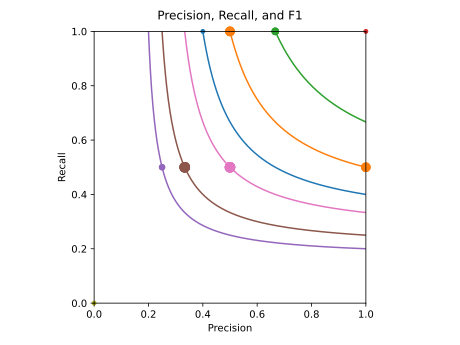
\includegraphics[width=0.6\textwidth]{images/scatter_precision_recall_f1.pdf}
\caption{F1 score isoquants showing how different combinations of precision and recall can yield the same F1 score. Each curve represents a constant F1 value.}
\label{fig:f1-isoquants}
\end{figure}

In \cref{fig:f1-isoquants}, it is clear that the green dot is better than the purple dot because it has both a better precision and recall score. Again, it's not obvious which orange dot is better. The F1 score takes a stance by saying they are tied. Notice the curvature of the F1 isoquants as well. The convexity of the region above the curve means that averages are preferred to extremes, roughly. Any dot on the line segment connecting the two orange dots would have a higher F1 score and thus correspond to a better model.


\subsubsection{Precision--Recall (PR) Curves}

The PR curve plots \emph{precision} (y-axis) against \emph{recall} (x-axis) as vary a model's decision threshold. Let the \emph{prevalence} be $\pi = \Pr(Y=1)$. Useful facts:
\begin{itemize}
\item At extreme low thresholds (label everything positive), recall $=1$ and precision $=\pi$.
\item A random classifier that ignores $X$ yields $\mathbb{E}[\text{precision at any recall}]=\pi$; its PR curve is a flat horizontal line at $y=\pi$.
\item Better-than-random models lie above the baseline for a wide range of recalls; higher \emph{area under the PR curve} (AUPRC) is better.
\item Threshold trade-off: increasing the threshold typically increases precision (fewer predicted positives) and decreases recall; lowering it does the opposite. PR is often more informative than ROC under class imbalance because the baseline and AUPRC depend on $\pi$.
\end{itemize}

\begin{figure}[H]
\centering
% requires \usepackage{tikz}
\begin{tikzpicture}[x=6cm,y=6cm]
  \def\prev{0.30} % prevalence \pi (shown for illustration)
  % axes
  \draw[->] (0,0) -- (1.05,0) node[below] {Recall};
  \draw[->] (0,0) -- (0,1.05) node[left] {Precision};
  % ticks
  \foreach \x/\lbl in {0/0,0.5/0.5,1/1} {
    \draw (\x,0) -- (\x,-0.015) node[below] {\small \lbl};
  }
  \foreach \y/\lbl in {0/0,0.5/0.5,1/1} {
    \draw (0,\y) -- (-0.015,\y) node[left] {\small \lbl};
  }
  % random baseline at prevalence
  \draw[dashed] (0,\prev) -- (1,\prev);
  \node[right] at (1,\prev) {\small random baseline $=\pi$};
  % an illustrative PR curve (monotonically decreasing in practice)
  \draw[thick]
    plot[smooth] coordinates {
      (0.05,0.95) (0.15,0.90) (0.30,0.80) (0.50,0.62)
      (0.70,0.50) (0.85,0.36) (1.00,\prev)
    };
  % threshold trade-off annotations
  \fill (0.30,0.80) circle (0.0075) node[above left] {\scriptsize high threshold};
  \fill (0.85,0.36) circle (0.0075) node[below right] {\scriptsize low threshold};

\end{tikzpicture}
\caption{Precision--Recall (PR) curve with random-classifier baseline at the prevalence $\pi$. Lower thresholds move rightward (higher recall) and typically downward (lower precision), illustrating the trade-off.}
\label{fig:pr-curve}
\end{figure}



\subsection{Experience and Training}

Our computer programs learn from \textit{experience} by being \textit{trained} on data. The training process involves adjusting model parameters to improve performance on the chosen metric.

In reality, the bail prediction problem faces a prohibitive missing data problem. In practice, we only observe outcomes for defendants who were actually released. We never learn what would have happened to those who were detained, so we can never obtain counts for true or false positives. Clever researchers work around this limitation. \cite{kleinberg2018human} exploits a natural experiment: comparing decisions by judges with different release tendencies to infer what might have happened in the counterfactual cases.

Moreover, our labels themselves are often proxies for what we really care about. When predicting ``crime,'' we typically observe arrests or convictions—not actual criminal behavior. Many crimes go unreported or unsolved. This means our training data, while probably useful, is not perfect.

As the statistician George Box famously said, ``All models are wrong, but some are useful.'' The question isn't whether our data perfectly captures reality (it doesn't), but whether our models can still provide valuable insights despite these limitations. In many cases, even imperfect predictions can improve upon human decision-making—as long as we remain clear-eyed about what our models can and cannot tell us. Finally, remember that your models cannot necessarily tell you anything without appropriate problem-specific knowledge. \cite{kuhn2013applied} discusses this in the introduction (Section 1.2).

\subsection{Summary}

We introduced the concept of a learning problem. This requires a performance measure and a way to use data (experience) to improve model performance. Prediction tasks are focal and when we have labeled data, we can use supervised learning techniques. We showed that the choice of a performance measure is (1) ambiguous because there are usually multiple plausible candidates and (2) substantive as it can lead you to prefer one model over the other. This highlights the \textbf{role of the researcher} in possessing problem-specific knowledge and technical knowledge. There is not generally a one-to-one mapping from learning tasks to particular models. The no free lunch theorems of \cite{wolpert1996lack} show that for any two learning algorithms, one won't outperform the other in all contexts, aligning with the agnostic approach to machine learning methods advocated by \cite{grimmer2021machine}. This places the burden on the researcher to understand and explore different models.
\newpage

% Chapter 2: Using LLMs  
\section{Using LLMs}

\begin{readingbox}
\begin{itemize}
\item Claude 4 Prompt Engineering Best Practices: \url{https://docs.anthropic.com/en/docs/build-with-claude/prompt-engineering/claude-4-best-practices}
\item OpenAI Prompt Engineering Guide: \url{https://platform.openai.com/docs/guides/prompt-engineering}
\end{itemize}
\end{readingbox}

LLMs are used in social science research for both classification (sentiment analysis, for example), document scaling, and topic modeling. The term ``foundation models'' is used to describe such general-purpose models. \cite{haaland2025understanding} highlights the use of LLMs to code open-ended data, noting LLMs will ``be the preferred choice over most existing text analysis methods for survey researchers.'' \cite{ornstein2025train} notes where LLMs underperform, though the analysis is limited to GPT-4 and GPT-3. Other methods might be preferred when high-quality training data is available or in the case of very large data where LLMs are expensive. What does very large mean? Using GPT-5 through OpenAI's API, it would cost maybe \$5 to classify 10,000 text responses of about 100 words.\footnote{\textit{Assumptions.} Model = GPT-5 API priced at \$1.25 per 1M \textbf{input} tokens and \$10.00 per 1M \textbf{output} tokens. Tokenization rule-of-thumb: \textbf{100 tokens $\approx$ 75 words} $\Rightarrow$ 100 words $\approx$ ~130 input tokens. Output kept minimal (label + brief rationale) at ~30 tokens. No few-shot examples; reusable instructions negligible and \textbf{no prompt caching} assumed. Per-response cost $\approx$ \(130 \times 1.25 \times 10^{-6} + 30 \times 1 \times 10^{-5} = \$4.625 \times 10^{-4}\). Totals: \textbf{10k} responses $\approx$ \textbf{\$4.63} (rounded to \textbf{\$5}); \textbf{1M} responses $\approx$ \textbf{\$462.5} (rounded to \textbf{\$500}). Costs scale linearly with tokens.} These costs scale linearly, so classifying 1,000,000 responses would cost \$500. More complicated prompting could triple the cost.\footnote{\textit{Assumptions.} Few-shot, no caching. A prompt includes the 130 input tokens \textit{and} a 200-token rubric with 500 tokens of examples. This modifies the previous calculation by now using 830 input tokens. We still assume 30 output tokens. Totals: \textbf{10k} responses $\approx$ \textbf{\$13.38}; \textbf{1M} responses $\approx$ \textbf{\$1338.00}.} One can save costs by switching to a cheaper model like GPT-5 nano, which is 20-25x cheaper than GPT-5, or using classical text analysis methods.

The LLM cost would likely be dwarfed by the general administrative costs of conducting any survey. For example, \cite{roberts2014structural} uses structural topic modeling to analyze open-ended survey responses from the American National Election Survey, which included 2,323 respondents. The LLM cost would be relatively trivial.

While creating and fine-tuning LLMs is beyond our scope, we'll use them to:
\begin{itemize}
\item Ease into coding
\item Explore performance measures for classification tasks
\item Practice effective prompting
\end{itemize}

If an LLM solves your problem adequately, there's no need for more complex ML approaches unless the size of the data makes the LLM route too costly.

\subsection{Is Using Pre-trained LLMs Machine Learning?}

This raises an interesting philosophical question, which we might file next to questions like, ``Is Katy Perry an Astronaut?''

\textbf{Traditional ML Classification:}
\begin{itemize}
\item You provide labeled data (experience E)
\item Train a model on your specific task (T)
\item Performance (P) improves with more of your data
\end{itemize}

\textbf{Using Pre-trained LLMs:}
\begin{itemize}
\item The model already learned from internet-scale text (someone else's E)
\item You craft prompts to apply its knowledge to your task
\item Model parameters do not change as you provide more data.
\end{itemize}

So is it machine learning? Yes, by Mitchell's definition. The learning happened during pre-training, not when you use it. So, using an LLM doesn't make you a machine learning engineer the same way using a chess engine doesn't make you an AI researcher. There is one wrinkle: the model's performance does improve when you provide clearer instructions or examples. An LLM will adapt to your task without changing its underlying knowledge. For practical, research purposes, this distinction doesn't matter. You're still solving classification problems, and you still need rigorous evaluation. Whether you trained the model or someone else did, the scientific method remains the same: define your task, measure performance, validate results.

\subsection{How LLMs Work}

How LLMs work is an overly ambitious title for this short section. They are next-token predictors, but that's not a useful description. Nobody really has a comprehensive answer to what LLMs are doing, at least according to Stuart Ritchie of Anthropic (\url{https://youtu.be/fGKNUvivvnc?si=6vHzbT3D7zb-maPl&t=13}). But here are some reasonable points to be made.

\textbf{The ``Old'' Approach (GPT-3.5 Era):}
\begin{itemize}
\item ``Like a fancy autocomplete,'' according to Peter Grabowski of Google
\item Statistical pattern matching from many examples
\item Role prompts (e.g., ``You are an MIT mathematician'') shifted probability distributions to improve the chances of the autocomplete being correct
\item Hypothesized sweet spot in detail and length of a prompt
\end{itemize}

\textbf{Modern Chain-of-Thought Models:}
\begin{itemize}
\item Built-in multi-step reasoning
\item Hidden ``thinking'' processes before output
\item Self-selected reasoning approaches
\item Role-playing prompts less effective
\end{itemize}

In a demonstration video, ChatGPT's o3 was asked how to get to Carnegie Hall. You can see the thinking process (at 8x speed), where o3 reasons through the intent of the question based on what it already knows. ChatGPT 5 Thinking will behave like o3.

\begin{quote}
\textbf{Video Demo:} See ChatGPT o3's thinking process in action: \\
\url{https://www.youtube.com/watch?v=_tGDS6g63So} \\
\textit{(Shows o3 reasoning through "How do you get to Carnegie Hall?" at 8x speed)}
\end{quote}

Claude Haiku or ChatGPT 4.5 are more likely to answer ``Practice, practice, practice.'' This answer is seemingly the best for a sophisticated autocomplete.

\subsubsection{Fancy Autocomplete and Bias}

Fancy autocompletes have their drawbacks and these garner a lot of attention. Namely, LLMs can forward whatever bias is in their training data (like any other model). As noted in \cite{atari2023humans}, LLMs are biased toward the psychology of people from WEIRD (Western, Educated, Industrialized, Rich, and Democratic) societies. LLMs exhibit human-like cognitive biases when trying to generate random sequences \cite{van2024random}. If you ask AI for a random number, some models disproportionately choose 42. Claude is especially bad at this, in my own experience. 42 is a salient number because of Douglas Adams's ``The Hitchhiker's Guide to the Galaxy.'' Its fans are overrepresented on the Internet and thus in training data. Similarly, LLMs can reproduce stereotypes. Companies devote enormous resources to mitigating these biases, but it is not a solved problem.

\begin{figure}[htbp]
    \centering
    \includegraphics[width=\linewidth]{images/claudehaiku-refusal-20250603.png}
    \caption{Response from Claude Haiku 3.5}
\end{figure}

\begin{figure}[htbp]
    \centering
    \includegraphics[width=0.6\linewidth]{images/claude-haiku35-20250603.png}
    \caption{Response from Claude Haiku 3.5}
\end{figure}

\subsection{Prompt Engineering Evolution}

Prompt engineering has evolved, meaning many of the self-anointed gurus on LinkedIn should probably be ignored. And instead of falling into the trap of trying to hit a moving target by stating best practices in the era of GPT-5, we'll only take the time to mention that prompting strategies, like role priming, that attempted to shift the model to a better probability distribution are no longer important.

\textbf{Less effective now:}
\begin{itemize}
\item Role priming (``You are an expert...'')
\item Explicit ``think step-by-step'' instructions
\item Confidence boosting
\item Mystical incantations
\end{itemize}

\textbf{Still valuable:}
\begin{itemize}
\item Clear problem specification
\item Relevant context and constraints
\item Examples of desired output format
\item Domain-specific information
\item Being smarter than the LLM because they still hallucinate
\end{itemize}

It used to be emphasized that LLM performance improves if the prompt included an example with the desired output, instead of merely giving instruction. A prompt with one example corresponds to a one-shot prompting strategy and mutatis mutandis for zero-shot and multi-shot. Something I haven't addressed above is if newer chain-of-thought models still improve with multi-shot prompting strategies. We'll test this for ourselves shortly.

\section{Evaluating LLM Classifications for Supervised Tasks}

\cite{gilardi2023chatgpt} showed that ChatGPT can outperform crowd workers (Mechanical Turk) on text annotation tasks. \cite{tornberg2024large} shows that GPT-4 outperforms even experts in annotating political social media messages. But how do we know this? How do we measure performance? And how do we find the best prompt? Instead of approaching this through prompt engineering principles, we'll tackle this in a data-driven way by \textit{trying stuff and seeing what works best}.

\subsection{Zero vs. Few Shots: What Does the Evidence Say?}

\begin{table}[H]
\centering
\begin{tabular}{llll}
\toprule
\textbf{Study} & \textbf{Model(s)} & \textbf{Task family} & \textbf{Main result} \\
\midrule
Brown et al. 2020 & GPT-3 & 42 NLP benchmarks & 0-shot < 1-shot < 16-shot (classic few-shot curve) \\
Kojima et al. 2022 & GPT-3 & Reasoning (GSM-8K) & Adding \textit{``Let's think step by step''} closes 60\% of gap to few-shot. \\
Wei et al. 2022 & PaLM-540B & Math, commonsense & 8-shot CoT boosts accuracy by up to 36 pp over plain few-shot. \\
Liyanage et al. 2024 & GPT-4 & Twitter stance & Zero-shot CoT matched 4-shot accuracy ($\approx$ 93\%). \\
Chen et al. 2024 & GPT-4 & 6 tasks & Extra demos show diminishing returns after coverage of each label. \\
\bottomrule
\end{tabular}
\caption{Research on zero-shot vs. few-shot prompting effectiveness}
\label{tab:few-shot-research}
\end{table}

Including examples should be less important in more modern models. You will test this in your homework.

\subsection{Exercises}

\begin{exercisebox}[title={LLM Classification Comparison}]
Find a labeled text data set of interest (here is one from \cite{liyanage2024gpt}: \url{https://github.com/Ravihari123/GPT-for-Twitter-Stance-Labeling/blob/main/final_annotated_dataset_355\%20records.csv}) with no more than 400 observations. Write two prompts for classification: one with two examples and one with no examples. Classify the entire data set using Gemini 2.5 Pro and then Gemini 2.5 Flash-Lite for a total of four ``models.'' Compare accuracy across each. You will be provided with an API key and some sample code.
\end{exercisebox}

\begin{exercisebox}[title={Grimmer Replication}]
Replicate \cite{grimmer2010bayesian} using an LLM. Find the data here: \url{https://github.com/lintool/GrimmerSenatePressReleases}.
\end{exercisebox}
\newpage

% Chapter 3: Predictive Modeling
\section{Predictive Modeling}

In this section we discuss the general predictive modeling process, model tuning, the problem of overfitting, and cross-validation. This draws mostly on \cite{kuhn2013applied} Chapters 2 and 4. However, I don't recommend any of the texts (APM, ESL, or ISL) for its treatment of cross-validation. Instead, consider the scikit-learn documentation (\url{https://scikit-learn.org/stable/modules/cross_validation.html}) or these lecture notes.

\subsection{Predicting $\hat{y}$}

Most of the machine learning models we will cover focus on prediction. In this world, we are not interested in marginal effects like the increase in wages attributable to schooling, standard errors, or even interpretability. Instead, we focus on some measure of predictive accuracy. A black box model is fine and a simpler model might only be preferred with parsimony as a tiebreaker.

\subsection{Tufte's Midterm Elections Model}

Let's focus on regression problems where $y$ is a continuous scalar value. For concreteness, let's say we are predicting midterm election vote share like in \cite{tufte1975determinants}. The $y$ variable is the percentage-point difference between the president's party's midterm two-party House vote share and that party's normal vote (average over the previous eight House elections).

\cite{tufte1975determinants} finds an equation 

\begin{equation}
\widehat{\mathrm{Vote\,Loss}} = -11.08 + 0.035\times \Delta\mathrm{Real\,Disposable\,Income} + 0.133\times \mathrm{Presidential\,Approval}
\label{eq:tufte-model}
\end{equation}

This line was found based on data from 1938-1970 and the R-squared is 0.912. Recall that R-squared describes how much of the variation in $y$ is captured by the model. A perfect model gives an R-squared of 1 and a model with only an intercept equal to the average of $y$ gives an R-squared of 0. Tufte's 0.912 is impressive. With intro stats training, you might only ask for the adjusted R-squared as a follow-up. The adjusted R-squared is also impressive at 0.876.

Adjusted R-squared is a blunt way to prevent being overconfident in your model. After all, we can add new features of random noise, uncorrelated to $y$ and improve the R-squared. With enough columns, the R-squared will become exactly 1. The adjusted R-squared formula essentially penalizes the R-squared based on the number of predictor variables and the number of observations.

However, the usefulness of this as a predictive model hinges on model performance on elections \textit{after} 1970. Evaluating the model on a \textbf{test set} of previously unseen data is more data driven and it answers the question of interest more exactly. The general principle is that a model should be evaluated with new data that wasn't used in the model training. Records from 1938-1970 form the \textbf{training set} and we can assemble data from 1974-2022 as a \textbf{test set}.

Let's see how two modifications of Tufte's model hold up with test data. I was unable to replicate Tufte's Real Disposable Income variable, so I substitute a similar RDI measure using data available from the BEA. In our model 1, we include only the presidential approval variable: \code{vote_loss ~ presidential_approval}. Model 2 is spiritually the same as Tufte's though: \code{vote_loss ~ change_rdi + presidential_approval}.

We will see that none of these models performs very well on the test data.

\begin{lstlisting}[language=Python]
# hide code and output
import pandas as pd
import numpy as np
import matplotlib.pyplot as plt
import statsmodels.formula.api as smf
import statsmodels.api as sm
from predictive import calculate_out_of_sample_r2

url = 'https://raw.githubusercontent.com/alexanderthclark/pols4728/refs/heads/main/data/tufte_midterms.csv'
df = pd.read_csv(url)

# Tufte analysis
tufte_model = smf.ols(formula='vote_loss ~ pres_approval + delta_rdi', data=df[df.in_original==True]).fit()
tufte_model_sub = smf.ols(formula='vote_loss ~ pres_approval + dpi_pc_pct_yoy', data=df[df.in_original==True]).fit()
out_of_sample_average = sm.OLS(df[df.year > 1970].vote_loss, np.ones(13)).fit()
tufte_approval_only = smf.ols(formula='vote_loss ~ pres_approval', data=df[df.in_original==True]).fit()

df['single_lin_reg_residuals'] = df.vote_loss - tufte_approval_only.predict(df.pres_approval)
df['multi_reg_residuals'] = df.vote_loss - tufte_model_sub.predict(df[['pres_approval', 'dpi_pc_pct_yoy']])
df['multi_reg_predictions'] = tufte_model_sub.predict(df[['pres_approval', 'dpi_pc_pct_yoy']])

df1 = df[df.in_original==True]
df2 = df[df.year > 1970]
\end{lstlisting}

\subsubsection{Model 1}

Model 1 has an R-squared of 0.253 in the training set. From the scatter plot below, we can see that the regression line is sane but imperfect when compared to the test data. The R-squared is just 0.015 on the test set. That means using the regression model is not much better than just guessing the average from the post-1970 data.


\begin{figure}[H]
\centering
\includegraphics[width=\textwidth]{images/model1_scatter.pdf}
\caption{Model 1: Presidential approval only. Left panel shows training data (blue) and test data (orange) with fitted regression line. Right panel shows residuals over time.}
\end{figure}

\subsubsection{Model 2}

Model 2 has an R-squared of 0.876 in the training set. From the residual scatter below, we see that the residuals become more volatile over time. Indeed, the R-squared is -0.233 (yes, negative) for the test data. That means using the regression model is worse than just guessing the average from the post-1970 data.

\begin{figure}[H]
\centering
\includegraphics[width=\textwidth]{images/model2_scatter.pdf}
\caption{Model 2: Presidential approval and economic indicator. Left panel shows predicted vs actual values for training and test data. Right panel shows residuals becoming more volatile over time.}
\end{figure}

\subsection{Could Tufte have produced a better model?}

Above we see that model 1 is actually better than model 2 on test data. This is a case where a simple model generalizes to new data better. Should Tufte have known this? Probably not. He didn't have access to the test data. To perform model selection, he would have needed to reserve some of his eight observations for validation. With more data, we should be able to do better. The next section tries to make that process more clear.

\section{Bias-Variance Tradeoff}

There is in general a tradeoff between a model's \textit{bias} and its \textit{variance}. Bias refers to the difference between the truth and what your model predicts. Variance refers to the tendency for the exact model fit to vary according to the randomness of the data you have. Both are bad. We like unbiased models and we want low variance so that our predictions are more exact.

More complicated models tend to have higher variance. As you add more features or polynomial terms to a linear regression, your model is more sensitive to noise. However, a more simplistic model won't come as close to describing the data generating process as it really is. Thus a simple model is biased.

When we decide on a performance metric like mean squared error (MSE) we are saying that we are willing to trade a reduction in one for an increase in the other. This is somewhat different than an emphasis on unbiased models (OLS is the BLUE) you might be familiar with in other settings.

\subsection{Bias–Variance Decomposition (supervised prediction)}

\textbf{Data-generating process}
\begin{itemize}
\item $Y = \theta + \varepsilon$
\item $\mathbb{E}[\varepsilon] = 0$, $\mathbb{Var}(\varepsilon) = \sigma^2$
\item $\hat \theta$ is an estimator (random through the training sample/algorithm)
\end{itemize}

Define the test MSE:

\begin{equation}
\mathrm{MSE} = \mathbb{E}\!\left[(Y - \hat \theta)^2\right]
\label{eq:mse-definition}
\end{equation}

Substitute $Y=\theta+\varepsilon$:

$$\begin{aligned}
\mathrm{MSE}
&= \mathbb{E}\!\left[(\theta+\varepsilon-\hat \theta)^2\right] \\
&= \mathbb{E}\!\left[(\theta-\hat \theta)^2\right] + \mathbb{E}[\varepsilon^2] + 2\,\mathbb{E}\!\left[\varepsilon\left(\theta-\hat \theta\right)\right).
\end{aligned}$$

Because $\mathbb{E}[\varepsilon]=0$ and the noise $\varepsilon$ is independent of the training randomness in $\hat \theta$, the cross term is $0$. Hence

$$\mathrm{MSE} \;=\; \underbrace{\mathbb{E}\!\left[(\theta-\hat \theta)^2\right]}_{\text{estimation error}}
\;+\; \underbrace{\sigma^2}_{\text{irreducible noise}}.$$

Now split the estimation error into $\mathrm{bias}^2$ and variance:

$$\begin{aligned}
\mathbb{E}\!\left[(\theta-\hat \theta)^2\right]
&= \mathbb{E}\!\left[(\hat \theta-\mathbb{E}[\hat \theta] + \mathbb{E}[\hat \theta]-\theta)^2\right] \\
&= \mathbb{E}\!\left[(\hat \theta-\mathbb{E}[\hat \theta])^2\right] + (\mathbb{E}[\hat \theta]-\theta)^2 + 2\,\mathbb{E}\!\left[(\hat \theta-\mathbb{E}[\hat \theta])(\mathbb{E}[\hat \theta]-\theta)\right] \\
\end{aligned}$$

The first term is the variance of $\hat{\theta}$ by definition. The second term is the squared bias, by definition. The last, cross term is zero (the second factor is constant with respect to the expectation over training randomness), so

$$\begin{aligned}
\mathbb{E}\!\left[(\theta-\hat \theta)^2\right] &= \underbrace{\mathbb{Var}(\hat \theta)}_{\text{variance}} + \underbrace{(\mathbb{E}[\hat \theta]-\theta)^2}_{\text{bias}^2},
\end{aligned}$$

Therefore,

\begin{equation}
\boxed{\ \mathrm{MSE} = \underbrace{(\mathbb{E}[\hat \theta]-\theta)^2}_{\text{bias}^2} + \underbrace{\mathbb{Var}(\hat \theta)}_{\text{variance}} + \underbrace{\sigma^2}_{\text{irreducible noise}}\ }
\label{eq:bias-variance-decomposition}
\end{equation}

\subsubsection{Interpretation}

\begin{itemize}
\item \textbf{Bias}: systematic error from model misspecification/rigidity.
\item \textbf{Variance}: sensitivity to the particular training sample.
\item \textbf{Noise}: randomness you cannot remove.
\end{itemize}

Making the model more flexible typically reduces bias but increases variance; restricting it does the opposite. Optimal predictive performance sits where $\mathrm{bias}^2$ + variance is minimized, as shown in \cref{eq:bias-variance-decomposition}.

\subsubsection{Examples}

Let $f(x) = \sin x + \varepsilon$, where $\varepsilon$ is normally distributed, iid noise. Suppose we observe $x$ drawn uniformly from $[0,\pi]$ so we only have the symmetric inverted-U shape.

\begin{figure}[H]
\centering
\includegraphics[width=\textwidth]{images/sine_examples.pdf}
\caption{Sine function examples showing bias-variance tradeoff between linear and quadratic models on different training datasets.}
\end{figure}

In the above, the simpler model will perform much better if the distribution of $x$ values shifts (technically called covariate shift), so that we start observing values $x>\pi$. The more complex, quadratic model is probably better in all other circumstances.

Sometimes the simpler model is better for any sample of $x$ values from the same distribution. This is a more pure bias variance tradeoff. Suppose instead the actual data generating process is one of pure noise $g(x) = \varepsilon$, but that there is a lot of noise so the standard deviation of the noise is high. The quadratic model is \textit{correctly specified} but, because it is so sensitive to the noise, it might not perform as well as the biased linear model with lower variance. Hence the tradeoff.

\begin{figure}[H]
\centering
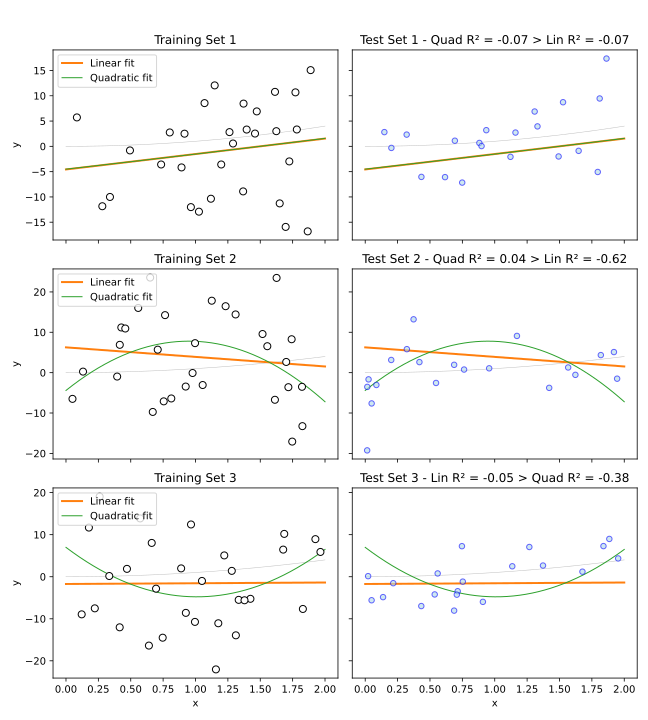
\includegraphics[width=\textwidth]{images/scatter_bias_variance.pdf}
\caption{Quadratic truth with noise showing training vs test performance for linear and quadratic models.}
\label{fig:bias-variance}
\end{figure}

\section{Validation and Model Selection}

We have seen how simple, biased models can sometimes generalize better than unbiased models. We have seen that complex models will fit our training data better but fail to perform well on test data. We have even critiqued Ed Tufte with the benefit of hindsight. Soon, it will be our turn to step into the arena and create our own models. Given that our goal is to produce a model that performs well on new data, we need to do our own validation that this will be the case. The way this is typically done is by \textbf{cross validation}. Cross validation has two uses:

\begin{enumerate}
\item Obtain a measure of the performance of your model
\item Tune your model's \textbf{hyperparameters}. This is called model selection.
\end{enumerate}

Hyperparameters are model parameters that need to be set by the researcher. Neural networks and other complex models involve many hyperparameters. If you are working with a fixed OLS specification, then there are no hyperparameters. The slope of a regression line is \textit{not} a hyperparameter, because it is determined by the model training process. However, we might consider the degree of polynomial that we use in a regression to be a hyperparameter.

\subsection{Simple Holdout Validation}

The most basic form of validation goes like this: randomly split the data into training, test, and a \textit{validation} (aka \textit{dev}) set. Then

\begin{enumerate}
\item Train each model variant (eg different polynomial specifications) on the training set.
\item Measure the error on the dev set.
\item Pick model with the lowest error on the dev set.
\item Reserve the test set to get a final measure of the model performance.
\end{enumerate}

One rule of thumb is to use 60\% of your data for training, 20\% for dev, and 20\% for test. With large data, you might keep more data for training. Large is relative to the size of an effect you're trying to detect, so we won't make this more precise for now.

This method enables us to perform model selection and to get an estimate of our model's error. You might find it striking that we \textit{make no decisions on the basis of the test set}. When data is scarce, this is obviously inconvenient. Why can't we use the dev set error to report on our model? Each measurement is a noisy read on the actual model performance. Once we select the model that looks the best on the dev set, we create some bias--we're selecting for models that perform very well by chance. Of course, we still want to select the model with the best performance, but we shouldn't be surprised if the model doesn't do quite as well on the test set. This phenomenon is sometimes referred to as \textit{model-selection bias}, an instance of the \textit{winner's curse}, or simply \textit{optimistic bias}.

Whenever you select for an extreme, you tend to end up capturing what might be some exceptional noise. As an analogy, consider all of the Forbes 30 Under 30 honorees who have gone to jail. By selecting for success, as it is noisily measured, Forbes ends up honoring a few people who are fraudsters or just very lucky (see Twyman's Law and regression to the mean).

\subsection{Cross Validation (For Model Performance)}

With scarce data and enough computing power, cross validation is often preferred, where we rotate the data through training and validation sets. Specifically in $\mathbf{k}$-\textbf{fold} validation,

\begin{enumerate}
\item Randomly split the data in $k$ partitions, or folds, of equal size.
\item Choose $k-1$ folds for training.
\item Use the remaining fold for validation--for a measure of performance.
\item Repeat 2-3 so that each fold is used as a validation set.
\item Compute the cross-validation estimate as the size-weighted mean of the fold-level validation errors. If folds are equal size, this reduces to the simple average.
\begin{equation}
\widehat{\mathrm{CV}}=\sum_{k=1}^K \frac{n_k}{N}\,\mathrm{Err}_k
\label{eq:cross-validation}
\end{equation}
\end{enumerate}

There is a sort of bias variance tradeoff in choosing $k$. If $k$ is small, your final performance estimate is pessimistic because the model is trained on relatively few data points. If $k$ is large (for instance, in the extreme of $k=n$, leave-one-out cross validation), then there is less bias but higher variance. $k$ between 5 and 10 is usually recommended.
   
This will generally give you a good measure of your model's performance on new data \textit{as long as you aren't using this for model selection.} \cite{varma2006bias} shows cross validation is biased in this case, though this isn't made especially clear in ESL and other texts.

\subsection{Nested Cross Validation (For Model Selection and Model Performance)}

In nested cross validation, we use two layers of cross validation: an inner loop for model selection (hyperparameter tuning) and an outer loop for performance estimation. This approach provides an unbiased estimate of model performance while avoiding the model-selection bias discussed previously.

The process works as follows:

\begin{enumerate}
\item \textbf{Outer Loop} (Performance Estimation):
   \begin{itemize}
   \item Split data into $K_{\mathrm{outer}}$ folds
   \item For each outer fold $k = 1, ..., K_{\mathrm{outer}}$:
     \begin{itemize}
     \item Hold out fold $k$ as the test set
     \item Use the remaining $K_{\mathrm{outer}} - 1$ folds for the inner loop
     \end{itemize}
   \end{itemize}

\item \textbf{Inner Loop} (Model Selection):
   \begin{itemize}
   \item Split the training data (from outer loop) into $K_{\mathrm{inner}}$ folds
   \item For each hyperparameter configuration:
     \begin{itemize}
     \item Perform $K_{\mathrm{inner}}$-fold cross validation
     \item Calculate average validation performance
     \end{itemize}
   \item Select the best hyperparameter configuration
   \item Retrain model with best hyperparameters on all inner loop data
   \end{itemize}

\item \textbf{Evaluation}:
   \begin{itemize}
   \item Test the model from step 2 on the held-out outer fold
   \item Repeat for all outer folds
   \item Report the average performance across all outer folds as the final estimate
   \end{itemize}
\end{enumerate}

Note, your average performance measure might average over models with different hyperparameter and can only be interpreted as the performance of your general algorithm.

In my experience in industry, a degenerate case of nested cross validation is the most common. $K_{\mathrm{outer}}$ is usually set to one, so this is just cross-validation over a training+dev set and with a test set that is left untouched until after you have selected your model. This also makes it easier to decide what hyperparameters you should actually pick if you're deploying a model.

\subsubsection{Why Nested Cross Validation?}

Using regular cross validation for both model selection and performance estimation leads to optimistic bias. When you select the best-performing model based on cross validation scores, you're essentially ``peeking'' at the test data through the selection process. The model that performs best might have gotten lucky with the particular data splits.

Nested cross validation separates these concerns:
\begin{itemize}
\item The inner loop finds the best hyperparameters for each outer training set
\item The outer loop provides an unbiased estimate of how well this model selection procedure works on truly unseen data
\end{itemize}

\subsection{Time Series, Unbalanced Data, and Other Complications}

For time series, the use of longitudinal holdouts are essential so that your validation and test sets contains data from a later time period than the data used for training.

\section{Summary}

We've now learned about the predictive modeling process. Model tuning and selection is prone to the problem of over-fitting. Performance measures like R-squared (and adjusted R-squared) are misleading when calculated based on training data. A model's performance can only truly be measured by using completely new test data that was not involved in the training process. The researcher needs to remain disciplined and use procedures like cross-validation to make model selection more systematic, transparent, and reliable. As noted by Susan Athey (\url{https://www.econtalk.org/susan-athey-on-machine-learning-big-data-and-causation/}), instead of researchers subjectively choosing variables and testing specifications behind the scenes, we can now explicitly use data to determine which variables matter. This technological shift enables what \cite{grimmer2021machine} describe as a move away from purely deductive social science toward a more inductive, iterative approach where researchers can discover patterns in data rather than only testing pre-specified hypotheses.

\section{Exercises}

\begin{tcolorbox}[breakable, size=fbox, boxrule=1pt, pad at break*=1mm,colback=cellbackground, colframe=cellborder, title=Exercise: Tufte Model Comparison]
Using \code{tufte_midterms.csv}, build a few models using data from 1970 and earlier. Compare the test R-squared for the different model specifications. What specification performs best?
\end{tcolorbox}

\begin{tcolorbox}[breakable, size=fbox, boxrule=1pt, pad at break*=1mm,colback=cellbackground, colframe=cellborder, title=Exercise: Cross-Validation Usage]
Lisa and Bart are trying to find the best model to predict the quantities of oil underground. Lisa chooses her model by (1) dividing her data into test and training. (2) She compares the performance of several different models and hyperparameter settings using 5-fold cross validation on the training set. Each model is trained five times and evaluated on the five different holdout folds. She obtains an estimate of the model performance by averaging over each of the five evaluations. (3) She picks the winning model and tuning parameters based on the CV procedure. (4) She uses the test set at the end to get a final measure of performance for the selected model.

Bart uses a similar procedure but he picks the winner by using the \textit{test} set. He uses CV to tune different types of models. Then, he compares each tuned model on the test set and picks the model with the best performance.

Who uses cross validation correctly? Lisa? Bart? Both? Neither?
\end{tcolorbox}

\begin{tcolorbox}[breakable, size=fbox, boxrule=1pt, pad at break*=1mm,colback=cellbackground, colframe=cellborder, title=Exercise: James-Stein Estimator]
Consider the estimator: $\theta_\alpha = (1 - \alpha)Y$, where $\alpha$ is a constant in $[0,1]$ and $Y\in \mathbb{R}^3$ is vector of independent normal random variables where $Y_i\sim N(\theta_i, 1)$ for $i=1,2,3$.

1.) Show that $\mathrm{MSE}(\alpha) = \mathbb{E}_Y \Vert \theta - \theta_\alpha \Vert^2  = \alpha^2 \Vert \theta \Vert^2 + 3(1-\alpha)^2 $

2.) Find the value of $\alpha$ that minimizes the MSE.

3.) Show the MSE-optimal $\theta_\alpha$ is also biased.
\end{tcolorbox}

\begin{tcolorbox}[breakable, size=fbox, boxrule=1pt, pad at break*=1mm,colback=cellbackground, colframe=cellborder, title=Exercise: P-hacking vs Overfitting]
In what ways are p-hacking and overfitting similar? In what ways are they different?
\end{tcolorbox}

% Print bibliography at the end
\newpage
\printbibliography

% Creative Commons license notice - REMOVED
% \vfill
% \doclicenseThis

\end{document}